\documentclass[a4paper,12pt]{scrbook}
\usepackage[utf8]{inputenc}
\usepackage[slovene]{babel}

\usepackage{amsmath}
\usepackage{amsfonts}
\usepackage{graphicx}
\usepackage{hyperref}



% Okolje za pisanje nalog
\usepackage{exercise}
%\usepackage[answerdelayed]{exercise}
\renewcommand{\ExerciseHeaderTitle}{~\textit{\ExerciseTitle}~~}
\renewcommand{\ExerciseHeaderNB}{\textsf{\textbf{\thechapter.\theExercise}}}
\renewcommand{\ExerciseHeader}{\par\noindent\ExerciseHeaderNB\ExerciseHeaderTitle}

\renewcommand{\AnswerHeader}{{\par\noindent\small\ExerciseHeaderNB}~}
\renewcommand{\AtBeginAnswer}{\footnotesize}

% Bližnjice
% exercise
\def\exe#1{\begin{Exercise}#1\end{Exercise}}
% exercise: +title
\def\exetit#1#2{\begin{Exercise}[title=#1]#2\end{Exercise}}
% exercise: +label
\def\exelbl#1#2{\begin{Exercise}[label=#1]#2\end{Exercise}}
% exercise: +title, +lable
\def\exetitlbl#1#2#3{\begin{Exercise}[title=#1,label=#2]#3\end{Exercise}}
% answer
\def\ans#1{\begin{Answer}#1\end{Answer}}
% reference to the exercise 
\def\refexe#1{$\rightarrow$\ref{#1}}
% algorithm name
\def\alg#1{\quot{#1}}

% Vrste nalog:
% * zgled (naloga + rešitev + pojasnilo)
% * naloga z namigom
% * naloga z rešitvijo
% * naloga (brez dodatkov)
% * izziv (težja naloga)
% * programerska naloga
% * sadistična naloga (npr. pointer na pointer na pointer na pointer, forktree pri OS)


\usepackage{xcolor}
\usepackage{listings,lstautogobble}
\lstset{frame=,
	language=Pascal,
	aboveskip=2mm,
	belowskip=2mm,
	showstringspaces=false,
	columns=flexible,
	basicstyle={\ttfamily},
	numbers=none,
	numberstyle=\tiny\color{gray},
	keywordstyle=\color{blue},
	morekeywords={downto,return},
	commentstyle=\color{gray},
	stringstyle=\color{green},
	breaklines=true,
	breakatwhitespace=true,
	tabsize=3,
%	backgroundcolor=\color{yellow},
    autogobble=true
}

% page layout
\textwidth 15cm


% % % % % % % % % % % % % % % % % % % % %


\def\angl#1{(angl. #1)}
\def\intro#1{\textit{#1}}
\def\vic#1{\emph{#1}}
\def\code#1{\textsf{#1}}
\def\quot#1{''#1``}

\def\NN{\ensuremath{\mathbb{N}}}
\def\ZZ{\ensuremath{\mathbb{Z}}}
\def\RR{\ensuremath{\mathbb{R}}}

\def\enumabc{\setlength{\itemsep}{0cm}\setlength{\parskip}{0cm}}


\renewcommand{\labelenumi}{\alph{enumi})}
\setlength{\parskip}{-0cm}


% % % % % % % % % % % % % % % % % % % % %

\begin{document}

\tableofcontents

\chapter{Problemi in algoritmi}

\section{Osnovni pojmi}

\exe{Zakaj je \vic{mestni} (arabski oz. indijski) zapis števil tako pomemben (tudi za algoritmiko)? Namig: predstavljajte si algoritem za seštevanje (ali pa množenje) rimskih številk.}


\exe{Kaj je \vic{število} \angl{number}, \vic{številka} \angl{numeral} in \vic{števka} \angl{digit}? In kaj je cifra in kaj mož?}


\exe{Kaj je bit in kaj je bajt? Kaj je več 42 kB ali 42 KiB? Koliko bitov je v 42 MiB?}


\exe{Od kje pride izraz \vic{algoritem}? S kakšnimi algoritmi se je ukvarjala dotična oseba?}


\exe{Opredeli (intuitivno, vendar natančno) pojem \vic{algoritma}. Obrazloži pomembne dele definicije.}


\exe{Sošolki povej en \vic{dvoumen} in en \vic{nejasen} stavek (vendar ne oboje). Kaj je težje sošolka ali stavek?}


\exe{Kaj je \vic{računski problem}? Podaj primer računskega problema, ki ni povezan z računanjem.}


\exe{Pojasni razliko med \vic{problemom} (kadar v algoritmiki rečemo problem imamo v mislih računski problem), \vic{nalogo} in \vic{rešitvijo}.}


\exe{Naštej in obrazloži vrste \vic{računskih problemov}: iskalni, odločitveni, preštevalni, naštevalni in optimizacijski. Za vsako vrsto podaj primer.}


\exe{Preveri veljavnost trditve:
\begin{enumerate}
\item Seštevanje, odštevanje, množenje dve števil so računski problemi, iskanje najmanjšega elementa v seznamu števil pa ni.
\item Za dana števila $x,y,z$ je vprašanje ali je $x+y=z$ odločitiveni problem.
\item Ali v danem seznamu elementov obstaja dani element je iskalni problem.
\item Urejanje seznama $5,2,9,3$ je računski problem.
\item Naloga problema poišči najbližjo točko koordinatnemu središču je seznam točk $(3,2), (1,5),(4,-2)$
\end{enumerate}
}


\exe{Zakaj je Turingov stroj pomemben za algoritmiko? Oglej si poljuben film o Alanu Turingu.}


\section{Snovanje in implementacija algoritmov}

\exe{Kaj je \vic{predpogoj} za dobro snovanje algoritmov?}
\ans{Dobro razumevanje problema preko natančne (matematične) definicije.}


\exe{Obrazloži nekaj kriterijev po katerih ocenjujemo kakovost algoritmov. Kateri kriterij je najpomembnejši?}
\ans{Pravilnost, učinkovitost, prilagodljivost, enostavnost, implementabilnost. Pravilnost je temelj vsakega algoritma.}


\exe{Naštej in primerjaj načine (\vic{opisni jeziki}) za opis algoritmov. Kateri načini so primernejši za ljudi in kateri za računalnike?}


\exe{Sošolki v naravnem jeziku obrazloži algoritem za iskanje največjega elementa v tabeli? Nato skupaj narišita diagram poteka za ta algoritem.}


\exe{Obrazloži faze razvoja algoritma od idejene zasnove do njegovega izvajanja. Obrazloži posamezne stopnje in semantične vrzeli med njimi. Kateri del je bolj abstrakten in kateri manj?}


\exe{Naštej nekaj pristopov oz. \vic{metod za snovanje} algoritmov. Več zabave s tem bo v sledečih poglavjih.}


\exe{Kaj je \vic{sintaktična} in kaj \vic{semantična} napaka v programu? Kaj je \vic{programski hrošč?}}


\exe{Naštej nekaj načinov za \vic{razhroščevanje} kode?}


\exe{Kaj je \vic{profiliranje} in kaj \vic{instrumentacija} kode?}


\exe{Kaj je sled algoritma?}


\exe{Ali za izvajanje algoritma vedno potrebujemo računalnik? Obrazloži.}


\section{Algoritmi od vsepovsod}


\exetitlbl{Največji in najmanjši element}{alg:minmax}{Zasnuj algoritme za iskanje največjega in najmanjšega elementa ter oboje hkrati. Kateri izmed algoritmov naredi manj primerjav elementov?}


\exetitlbl{Zaporedno iskanje}{alg:seqsearch}{Zasnuj algoritem za iskanje danega elementa v dani tabeli. V čem je razlika v nalogi tega problema v primerjavi s problemom \quot{največji in najmanjši element} iz predhodne naloge?}


\exetit{Ugani število}{S sošolko igrajta igro \quot{ugani število}: zamisli si število med 1 in 128, ona pa naj ugiba, možni odgovori so manjše, enako, večje. Koliko ugibanj potrebuje v najslabšem primeru v različnih pristopih, npr. zaporedno iskanje, razpolavljanje (bisekcija).}


\exe{Načelo razpolavljanja (bisekcija) je eno izmed najbolj uporabnih načel v algoritmiki (in življenju nasploh). Kje se še uporablja?}
 

\exetitlbl{Dvojiško iskanje}{alg:binsearch}{Zasnuj algoritem \vic{dvojiško iskanje}, ki uporablja načelo razpolavljanja, za iskanje števila v urejenem zaporedju. V čem je razlika med nalogo tega problema in nalogo problema \quot{zaporedno iskanje} iz naloge \refexe{alg:seqsearch}? Zapiši tako rekurzivno kot iterativno obliko algoritma.}


\exetitlbl{Množenje s prištevanjem}{alg:mul-with-add}{Zasnuj algoritem za množenje dveh števil preko prištevanja. Namig: pomagaj si z definicijo množenja $a\cdot b = \underbrace{b + b + \dots + b}_{a-\text{krat}}$.}


\exe{Kdo je bil Evklid iz Aleksandrije? S čim se je še ukvarjal poleg algoritmov?}


\exe{Opiši \vic{Evklidov algoritem} za iskanje \vic{največjega skupnega delitelja}. Zapiši tako rekurzivno kot iterativno obliko algoritma.}


\exe{Opiši še en algoritem za iskanje \vic{največjega skupnega delitelja}, ki deluje preko faktorizacije števil.}


\exe{Prikaži sled Evklidovega algoritma za števili a) 123 in 456, b) 321 in 654 ter b) 59 in 61.}
\ans{a) \begin{tabular}{lllll}
\# & a & b & q & r \\
\hline
0 & 123 & 456 0 & 123 \\
1 & 456 & 123 & 3 & 87 \\
2 & 123 & 87 & 1 & 36 \\
3 & 87 & 36 & 2 & 15 \\
4 & 36 & 15 & 2 & 6 \\
5 & 15 & 6 & 2 & 3 \\
6 & 3 & 2 & 0 \\
7 & 3 & 0 \\
\end{tabular}}


\exe{Kaj se zgodi po prvem koraku Evklidovega algoritma, če je prvo število manjše od drugega?}


\exe{S pomočjo \vic{Eratostenovega sita} izračunaj praštevila manjša od $N=42$.}


\exetit{Faktoriela}{Zapiši rekurzivni algoritem za izračun faktoriele glede na formulo $n!=n\cdot(n-1)!$ in $0!=1$. Ali je algoritem vsebuje repno rekurzijo? Če ne, ga spremeni, da jo bo, nato pa vse skupaj spremeni v iteracijo. Opazuj spremembe!}
\ans{fun fac(n) is if n==0 then 1 else n*fac(n-1); fun factail(r, n) is if n==0 then r else factail(r*n,n-1).}


\section{Preverjanje pravilnosti}

\exe{Na svetovnem spletu poišči nekaj primerov znanih programskih hroščev.}


\exe{Kaj je poglavitno vprašanje (intuitivno), ki si ga postavimo, ko preverjamo pravilnost nekega algoritma?}
\ans{Ali program deluje, kot mislimo, da bi moralo delovati?}


\exe{Naštej (štiri) načine s katerimi lahko preverjamo pravilnost algoritmov.}


\exe{Utemelji pravilnost algoritma \quot{množenje s prištevanjem} (glej nalogo \refexe{alg:mul-with-add}) preko \vic{intuitivnega razumevanja}. Ali algoritem deluje za negativna števila?}


\exe{Zakaj se pri razvoju programov zelo pogosto uporablja testiranje s testnimi primeri? Zakaj za testiranje algoritmov to pogosto ni zadostno?}


\exe{Koliko različnih vhodov je možnih za Evklidov algoritem, če privzamemo 32-bitna števila? Koliko let bi trajalo popolno testiranje algoritma, če imamo na voljo testni sistem, ki vsako sekundo preizkusi miljardo ($10^9$) vhodov?}
\ans{Št. vhodov: $2^{64}\approx1,8\cdot 10^{19}$, čas testiranja: $2^{64} / 10^9 / 60 / 60 / 24 / 365 = 585$ let.}


\exe{Dano je polje dolžine 200. Tina Sredinec je implementirala algoritem, ki izračuna sredinsko pozicijo $m$ v polju med pozicijama $l$ (leva meja) in $r$ (desna meja), po formuli $m = (l+r)/2$. Vse spremenljivke vsebujejo 8 bitna nepredznačena števila. Kje se skriva programski hrošč? Kako bi program popravil?}
\ans{Za $l=150$ in $r=190$ dobimo $l+r=340 (\bmod 256)=84$ in torej $m=(l+r)/2=42$, kar očitno ni sredina med 150 in 180. Popravek: $m=l+(r-l)/2$.}


\exe{Ugotoviti želimo pravilnost nekega algoritma za urejanje seznama. Kateri dve lastnosti moramo preveriti?}
\ans{Da rezultat vsebuje enake elemente kot vhodno zaporedje in da je rezultat urejen seznam.}


\exe{V čem je prednost \vic{formalnega dokazovanja pravilnosti} algoritmov. Na katerem matematičnem načelu sloni dokazovanje pravilnosti algoritmov, ki vsebujejo zanke?}
\ans{Zanesljivost pravilnosti, indukcija.}


\exe{Formalni dokaz pravilnosti algoritma pogosto temelji na indukciji. Kaj je \vic{matematična indukcija}, \vic{hipoteza}, \vic{osnovni primer}, \vic{induktivna predpostavka} in \vic{induktivni korak}? V algoritmiki pa za dokazovanje zank uporabljamo tudi \vic{zančne invariante}.}


\exe{S pomočjo matematične indukcije dokaži $\sum_{i=0}^{n}i=\frac{n(n+1)}{2}$.}


\noindent\begin{minipage}{7.5cm}
\exe{S pomočjo indukcije dokaži pravilnost algoritma za iskanje maksimuma v tabeli števil.}
\end{minipage}
\hspace{1em}
\begin{minipage}{7cm}
\vspace{1.2em}
\begin{lstlisting}
m = a[0]
for i = 1 to n-1 do
	if a[i] > m then m = a[i]
\end{lstlisting}
\end{minipage}


\exe{S pomočjo indukcije dokaži pravilnost \quot{množenja s prištevanjem}.}


\exe{Dokaži pravilnost Evklidovega algoritma. Uporabite znani izrek v zvezi s tem.}

\chapter{Zahtevnost algoritmov}

\section{Splošna vprašanja}

\exe{Kaj je zahtevnost algoritma?}
\ans{Zahtevnost algoritma pove katere in koliko virov potrebuje algoritem za svoje izvajanje (v nekem modelu računanja).}


\exe{Naštej nekaj virov, ki jih algoritem lahko potrebuje za svoje izvajanje.}


\exe{Kateri viri ustrezajo meri \vic{časa} in kateri \vic{prostora}?}


\exe{Kaj je \vic{Von Neumannov} model računalniške arhitekture?}


\exe{Kaj je RAM model računanja? Zakaj ga uporabljamo v algoritmiki?}


\exe{Kaj je natančna zahtevnost in kaj asiptotična zahtevnost algoritma?}


\exe{Od česa je lahko odvisna zahtevnost algoritma? Prikaži s primerom.}
\ans{Od algoritma, modela računanja in od velikosti vhoda in samih podatkov v vhodu.}


\exe{Izberi nek problem, nato naštej nekaj primerov nalog zanj, katerih težavnost je različna:
\begin{enumerate}
\item glede na velikost naloge
\item glede na podatke v sami nalogi.
\end{enumerate} }


\exe{Glede na (vhodne) podatke, katere vrste določanja zahtevnosti poznamo?}


\exe{Zakaj najpogosteje uporabljamo zahtevnost v najslabšem primeru?}


\exe{Kdo je bil John von Neumann? S čim vsem se je ukvarjal? Katere izmed algoritmov za urejanje je napravil?}


\section{Natančna zahtevnost}


\exe{Koliko korakov zahteva algoritem \quot{množenje s prištevanjem} (glej nalogo \ref{alg:mul-with-add})?}


\exe{Koliko korakov zahteva Eratostenovo sito za poljuben $N$? En korak je mišljen kot odstranjevanje večkratnikov nekega števila $X$.}
\ans{Odstranjevanje večkratnikov $X$ je potrebno do: hitro vidimo, da za $X<N$ ali tudi $X<N/2$. Z malo razmislega pa pridemo do $X\leq\sqrt{N}$.}


\noindent\begin{minipage}{7.5cm}
\exe{Določi natančno zahtevnost v številu primerjav elementov glede na najboljši, najslabši in povprečni primer za algoritem (zaporednega iskanje, glej \refexe{alg:seqsearch}). Pri tem je $n$ velikost polja $a$.}
\end{minipage}
\hspace{1em}
\begin{minipage}{7cm}
\vspace{1.2em}
\begin{lstlisting}
for i = 0 to n-1 do
	if a[i] == key then return i
return -1
\end{lstlisting}
\end{minipage}
\ans{Najboljši primer: 1, najslabši primer: $n$ in povprečni primer $(n+1)/2$.}


\exe{Zakaj se kot pomembna operacija, s katero ocenjujemo zahtevnost, pogosto pojavi primerjava elementov, primerjavo indeksov pa navadno zanemarimo?}


\exe{Določi natančno zahtevnost v smislu realnega časa na poljubnem RAM modelu računanja za algoritem \quot{zaporedno iskanje} iz naloge \refexe{alg:seqsearch}}
\ans{Najboljši primer: $c_1+c_2+c_3$, najslabši primer: $c_1\cdot(n+1)+c_2\cdot n+c_3$, povprečni primer: $\frac{c_1+c_2}{2}n+\frac{c_1+c_2}{2}+c_3$, kjer je $c_1$ zahtevnost preverjanja pogoja v odločitvenem stavku, $c_2$ cena primerjave elementov in $c_3$ cena stavka return.}


\exe{Kolikšna je globina rekurzije pri algoritmu \alg{dvojiškega iskanja}?}


\section{Asimptotična zahtevnost}

\section{Namigi in rešitve izbranih nalog}

\shipoutAnswer

\chapter{Osnovne podatkovne strukture}


\section{Sklad}

\exe{Profesor Mate Matik želi preveriti ali je dano zaporedje oklepajev pravilno gnezdeno. Na primer npr. \code{()([])} in \code{()[\{(()[])\}]} sta pravilno gnezdeni zaporedji, \code{(()[]\}} in \code{(([()])}  pa nista. Pomagaj mu in zasnuj algoritem za ta problem.}

\exe{Kvantni fiziki iz Palindromije so izdelali novo vrsto naprave, ki generira številčne nize naključnih palindormov. Na voljo je le operacija \code{next()}, ki vrne naslednji znak palindorma oz. -1, če je palindroma konec. Na voljo imaš le en sklad in vrsto, zasnuj algoritem, ki preveri ali naprava res generira palindrom.}


\section{Povezani seznami}

\def\e#1{\id{enqueue(#1)}}
\def\d{\id{dequeue}}
\def\p#1{\id{push(#1)}}
\def\pop{\id{pop}}
\def\t{\mbox{}\quad\quad}
\exe{Enojno povezani seznam zaporedoma vsebuje elemente $3,0,4,1,5$.
\begin{enumerate}
\item Seznam uporabimo kot vrsto in nad njim izvedemo naslednje operacije: \d, \d, \e{9}, \e{2}, \d, \e{6}. Kakšen seznam dobimo?
\item Seznam uporabimo kot sklad in nad njim izvedemo naslednje operacije: \pop, \pop, \p{9}, \p{2}, \pop, \p{6}. Kakšen seznam dobimo?
\item Uporabite predstavitev seznama s poljem kapacitete 8, pri čemer naj bo element $i$ hranjen na indeksu $i$. Namig: zapišite polji \id{item} in \id{next} ter vrednosti \id{first} in \id{free}. 
\item Zapišite funkcijo \id{podvoji()}, ki podvoji kapaciteto seznama (predstavljenega s poljem). 
\end{enumerate}}
\ans{a) 1,5,9,2,6 b) 6,9,4,1,5 pri obeh a) in b) smo upoštevali tudi, če ste dodajali/odvzemali z nasprotnega konca
c) item: 0,1,-,3,4,5,-,- next: 4,5,6,0,1,-1,7,-1, first=3, free=2, d) Zanimivi del programa je del, ki popravi seznam prostih celic. Samo kopiranje elementov ni tako zanimivo.}


\section{Drevesa}

\exe{Celovito drevo stopnje tri je implicitno predstavljeno s poljem $3,1,4,1,5,9,2,6,5,3,5$.
\begin{enumerate}
	\item Nariši drevo.
	\item Zapiši enačbe za indekse vseh otrok vozlišča z indeksom $i$.
	\item Zapiši zaporedje vozlišč drevesa, če izvedemo premi obhod drevesa.
\end{enumerate}}
\ans{a) Drevo narišemo po nivojih. b) $3i+1, 3i+2, 3i+3$, c) 3,1,5,9,2,4,6,5,3,1,5}


\exe{Dano je naslednje drevo.\\
\begin{tabular}{ccc}
	\parbox{9cm}{
		\begin{enumerate}
			\item Zapiši stopnjo drevesa.
			\item Najmanj koliko vozlišč bi moral dodati, da bi drevo postalo polno?
			\item Zapiši vrstni red vozlišč pri obratnem obhodu drevesa.
	\end{enumerate}}
	&
	~
	&
	\parbox{5.5cm}{
		\tikzstyle{level 1}=[sibling distance=8em] 
		\tikzstyle{level 2}=[sibling distance=3em] 
		\tikzstyle{level 3}=[sibling distance=3em] 
		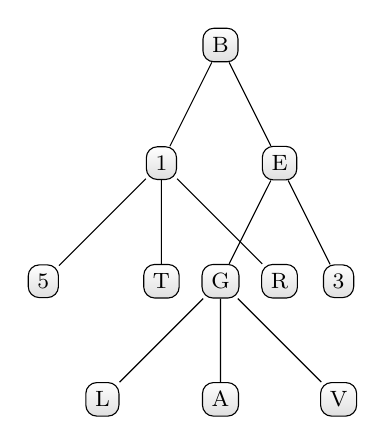
\begin{tikzpicture}[every node/.style = {shape=rectangle,rounded corners,draw, align=center, top color=white, bottom color=gray!25, font=\footnotesize}]]
		\node {B}
		child { node {1}
			child { node {5} }
			child { node {T} }
			child { node {R} }
		}
		child { node {E}
			child { node {G}
				child { node {L} }
				child { node {A} }
				child { node {V} }
			}
			child { node {3} }
		};
		\end{tikzpicture}}
\end{tabular}}
\ans{a) 3, b) 2, c) 5TR1LAVG3EB}


\exe{Gradnja min kopice z zaporednim vstavljanjem.
\begin{enumerate}
	\item Zgradi min kopico z zaporednim vstavljanjem števil iz naslednjega zaporedja
	$$ 9,3,1,9,7,6,2,7,5. $$
	Izriši drevo vsakič, ko vstaviš element v kopico. Jasno označi kopice.
	\item Koliko (natančno) zamenjav se opravi v \textbf{najslabšem} primeru in koliko v \textbf{najboljšem} primeru pri vstavljanju $i$-tega elementa? Namig: elemente začni šteti z 1.
	\item Zapiši primer zaporedij dolžine pet, kjer pride do najslabšega in do najboljšega primera.
	\item Zapiši asimptotično časovno zahtevnost v najslabšem primeru za takšen način gradnje.
	\item Zapiši algoritem, ki v konstantnem času vrne \textbf{drugi} najmanjši element kopice.
\end{enumerate}}
\ans{a) 3 b) 3 c) 2 d) 2}


\section{Namigi in rešitve izbranih nalog}

\shipoutAnswer
\chapter{Urejanje in izbiranje}


% a-izbrani element, b-mesto kamor postavimo izbrani element
\def\a#1{\textbf{#1}}
\def\b#1{\underline{#1}}


\setlength{\parindent}{0.0cm}
%\hangindent=0.5cm
\section{Navadna urejanja}

\intro{Pod navadna urejanja sodijo \vic{navadno izbiranje} \angl{selection sort}, \vic{navadne zamenjave}, imenovano tudi urejanje z mehurčki \angl{bubble sort}, in \vic{navadno vstavljanjem} \angl{insertion sort}.}

% ukazi za oznake v sledeh urejanja
\def\m#1{\textbf{#1}}
\def\b{\hfil\kern\arraycolsep\vline\kern-\arraycolsep\hfilneg}


\exetit{Navadno izbiranje}{Zapiši sled urejanja z navadnim izbiranjem v nepadajočem vrstnem redu za vhodno zaporedje $3,2,8,9,1,5,4,6,0,7$.}
\ans{\vtop{\vskip-1em
\begin{tabular}{l||llllllllllll}
  & \b & 3 & 2 & 8 & 9 & 1 & 5 & 4 & 6 & \m0 & 7 \\
\hline
0 & & 0 \b & 2 & 8 & 9 & \m1 & 5 & 4 & 6 & 3 & 7 \\
1 & & 0 & 1 \b & 8 & 9 & \m2 & 5 & 4 & 6 & 3 & 7 \\
2 & & 0 & 1 & 2 \b & 9 & 8 & 5 & 4 & 6 & \m3 & 7 \\
3 & & 0 & 1 & 2 & 3 \b & 8 & 5 & \m4 & 6 & 9 & 7 \\
4 & & 0 & 1 & 2 & 3 & 4 \b & \m5 & 8 & 6 & 9 & 7 \\
5 & & 0 & 1 & 2 & 3 & 4 & 5 \b & 8 & \m6 & 9 & 7 \\
6 & & 0 & 1 & 2 & 3 & 4 & 5 & 6 \b & 8 & 9 & \m7 \\
7 & & 0 & 1 & 2 & 3 & 4 & 5 & 6 & 7 \b & 9 & \m8 \\
8 & & 0 & 1 & 2 & 3 & 4 & 5 & 6 & 7 & 8 \b & 9 \\
\end{tabular}}}


\exe{Zapiši sled urejanja z navadnim izbiranjem v nenaraščajočem vrstnem redu za vhodno zaporedje $3,2,8,9,1,5,4,6,0,7$.}


\exe{Koliko primerjav in zamenjav naredi navadno izbiranje na vhodnem zaporedju a) $0,1,2,3,4,5,6,7,8,9$ in koliko na zaporedju b) $9,8,7,6,5,4,3,2,1,0$?}


\exe{Koliko natančno primerjav $C(n)$ naredi navadno izbiranje na zaporedju velikosti $n$?}
\ans{\vspace{-1em}$$ C(n) = \sum_{i=0}^{n-2} \sum_{j=i+1}^{n-1} 1 = \sum_{i=0}^{n-2} (n-i-1) = \sum_{i=1}^{n-1} i = \frac{n(n-1)}{2}. $$}


\exe{Koliko asimptotično primerjav $C(n)$ naredi navadno izbiranje na zaporedju velikosti $n$? Odgovor zapiši tako s pomočjo tilda kot $\Theta$ notacije.}
\ans{\vspace{-1em}$$ C(n) \sim \frac{n^2}{2} = \Theta(n^2). $$}


\exe{Koliko (natančno in asimptotično) zamenjav $S(n)$ naredi navadno izbiranje na zaporedju velikosti $n$?}
\ans{\vspace{-1em}$$ S(n) = n-1 \sim n = \Theta(n). $$}


\exe{Navadno izbiranje izboljšamo tako, da na vsakem koraku hkrati poiščemo najmanjši in največji element v še neurejenem delu zaporedja. Nato oba elementa postavimo (zamenjava) na ustrezno mesto. Zapiši sled urejanja za zaporedje $$3,2,8,9,1,5,4,6,0,7.$$}
\ans{\vtop{\vskip-1em
\begin{tabular}{l||llllllllllll}
  & \b & 3 & 2 & 8 & \m9 & 1 & 5 & 4 & 6 & \m0 & 7 \b \\
\hline
0 & & 0 \b & 2 & \m8 & 7 & \m1 & 5 & 4 & 6 & 3 \b & 9 \\
1 & & 0 & 1 \b & 3 & \m7 & \m2 & 5 & 4 & 6 \b & 8 & 9 \\
2 & & 0 & 1 & 2 \b & \m6 & \m3 & 5 & 4 \b & 7 & 8 & 9 \\
3 & & 0 & 1 & 2 & 3 \b & \m4 & \m5 \b & 6 & 7 & 8 & 9 \\
4 & & 0 & 1 & 2 & 3 & 4 \b\b & 5 & 6 & 7 & 8 & 9 \\
\end{tabular}}}


\exe{Na voljo imate algoritem za hkratno iskanje najmanjšega in največjega elementa, ki v zaporedju dolžine $n$ porabi $2n-2$ primerjav. Koliko natančno primerjav porabi s tem algoritmom izboljšano navadno izbiranje?}
\ans{\vspace{-1em}$$ C(n) = \sum_{i=0}^{\frac{n-2}{2}} (2(n-2i)-2) = \frac{n(n+2)}{2}-2. $$}


\exe{Na voljo imate algoritem za hkratno iskanje najmanjšega in največjega elementa, ki v zaporedju dolžine $n$ porabi $3/2n-2$ primerjav. Koliko natančno primerjav porabi s tem algoritmom izboljšano navadno izbiranje?}
\ans{$$ C(n) = \sum_{i=0}^{\frac{n-2}{2}} (n-2i) = \sum_{i=2}^{n} 2i $$.}


\exe{Navadno izbiranje želimo implementirati na enojno povezanem seznamu? Kolikšna je asimptotična časovna zahtevnost takega algoritma?}
\ans{$\Theta(n^2)$. Najmanjši elementi si zapomnimo v kazalcu min. Zamenjavo izvedemo tako, da zamenjamo elementa (ne prevezujemo vozlišč).}


\exetit{Navadne zamenjave}{Zapiši sled urejanja z navadnimi zamenjavami v nepadajočem vrstnem redu za vhodno zaporedje $3,2,8,9,1,5,4,6,0,7$.}
\ans{\vtop{\vskip-1em
\begin{tabular}{l||llllllllllll}
0 & \b & 3 & 2 & 8 & 9 & 1 & 5 & 4 & 6 & 0 & 7 \\
1 & & 0 \b & 3 & 2 & 8 & 9 & 1 & 5 & 4 & 6 & 7 \\
2 & & 0 & 1 \b & 3 & 2 & 8 & 9 & 4 & 5 & 6 & 7 \\
3 & & 0 & 1 & 2 \b & 3 & 4 & 8 & 9 & 5 & 6 & 7 \\
3 & & 0 & 1 & 2 & 3 \b & 4 & 5 & 8 & 9 & 6 & 7 \\
4 & & 0 & 1 & 2 & 3 & 4 \b & 5 & 6 & 8 & 9 & 7 \\
5 & & 0 & 1 & 2 & 3 & 4 & 5 \b & 6 & 7 & 8 & 9 \\
6 & & 0 & 1 & 2 & 3 & 4 & 5 & 6 \b & 7 & 8 & 9 \\
7 & & 0 & 1 & 2 & 3 & 4 & 5 & 6 & 7 \b & 8 & 9 \\
8 & & 0 & 1 & 2 & 3 & 4 & 5 & 6 & 7 & 8 \b & 9 \\
\end{tabular}}}


\exe{Zapiši sled urejanja z navadnimi zamenjavami v nenaraščajočem vrstnem redu za naslednje vhodno zaporedje $3,2,8,9,1,5,4,6,0,7$.}


\exe{Urejanje z navadnimi izmenjavami izboljšamo tako, da v postopek končamo, če v zadnji iteraciji ni prišlo do nobene zamenjave. Takšen postopek pravilno uredi poljubno zaporedje? Utemelji.}


\exe{Urejanje z navadnimi izmenjavami izboljšamo tako, da v naslednji iteraciji delamo primerjave le do indeksa zadnje zamenjave na predhodni iteraciji.}


\exetit{Navadno stresanje}{TODO: Shaker sort - navadno stresanje - sled}


\exetit{Navadno vstavljanje}{Zapiši sled urejanja z navadnimim vstavljanjem v nepadajočem vrstnem redu za vhodno zaporedje $3,2,8,9,1,5,4,6,0,7$.}
\ans{\begin{tabular}{l||lllllllllll}
i & \\
\hline
  & 3 \b & 2 & 8 & 9 & 1 & 5 & 4 & 6 & 0 & 7 \\
1 & 2 & 3 \b & 8 & 9 & 1 & 5 & 4 & 6 & 0 & 7 \\
2 & 2 & 3 & 8 \b & 9 & 1 & 5 & 4 & 6 & 0 & 7 \\
3 & 2 & 3 & 8 & 9 \b & 1 & 5 & 4 & 6 & 0 & 7 \\
4 & 1 & 2 & 3 & 8 & 9 \b & 5 & 4 & 6 & 0 & 7 \\
5 & 1 & 2 & 3 & 5 & 8 & 9 \b & 4 & 6 & 0 & 7 \\
6 & 1 & 2 & 3 & 4 & 5 & 8 & 9 \b & 6 & 0 & 7 \\
7 & 1 & 2 & 3 & 4 & 5 & 6 & 8 & 9 \b & 0 & 7 \\
8 & 0 & 1 & 2 & 3 & 4 & 5 & 6 & 8 & 9 \b & 7 \\
9 & 0 & 1 & 2 & 3 & 4 & 5 & 6 & 7 & 8 & 9 \b \\
\end{tabular}}


\exe{Katera izmed osnovnih navadnih urejanj v tem razdelku so stabilna? Utemelji!}
\ans{\begin{itemize}
	\item Navadno izbiranje: ni stabilno, protiprimer $2,2,1$;
	\item navadne zamenjave: je stabilno, enaki elementi se ne zamenjajo;
	\item navadno vstavljanje: je stabilno, vstavljamo kvečjemju do enakega elementa.
\end{itemize}}


\exetit{Črno beli diski}{TODO: Levitin p.102. Danih je $2n$ diskov dveh barv: $n$ črnih in $n$ belih. Bele želimo spravit na levi konec in črna na desni konec. Dovoljena operacija je edino zamenjava dveh sosednjih diskov. Zasnuj algoritem za reševanje tega problema in določi število potrebnih zamenjav.}
\ans{Uporabi navadne zamenjave ali navadno vstavljanje.}


\section{Napredna urejana}

\intro{V tem razdelku se lotimo algortimov za urejanje, katerih časovna zahtevnost je boljša od kvadratne.}

\exe{Izračunaj delilno zaporedje za \vic{Shellovo urejanje} zaporedja 3141 števil, če je število zunanjih iteracij algoritma enako $t=\lfloor\log_2 n\rfloor -1$ in $h_t=1$ ter $h_{k-1}=2h_k+1$.}
\ans{Število iteracij $t=10$ in delilno zaporedje je $(1023,511,255,127,63,31,15,7,3,1)$.}


\exe{Uredi zaporedje $3, 1, 4, 1, 5, 9, 2, 6, 5, 3, 5, 8, 9, 7, 9, 3, 2, 3, 8, 4, 6$ s Shellovim urejanjem v naraščajočem vrstnem redu.}
\ans{$t=3$, delilno zaporedje $(7,3,1)$.\\
\begin{tabular}{c|ccccccccccccccccccccc}
 h & ;3 & 1 & 4 & 1 & 5 & 9 & 2 & 6 & 5 & 3 & 5 & 8 & 9 & 7 & 9 & 3 & 2 & 3 & 8 & 4 & 6 \\
\hline
 7 & ;3 & 1 & 2 & 1 & 5 & 4 & 2 & 6 & 3 & 3 & 3 & 8 & 9 & 6 & 9 & 5 & 4 & 5 & 8 & 9 & 7 \\
 3 & ;1 & 1 & 2 & 2 & 3 & 3 & 3 & 4 & 4 & 3 & 5 & 5 & 5 & 6 & 7 & 8 & 6 & 8 & 9 & 9 & 9 \\
 1 & ;1 & 1 & 2 & 2 & 3 & 3 & 3 & 3 & 4 & 4 & 5 & 5 & 5 & 6 & 6 & 7 & 8 & 8 & 9 & 9 & 9 \\
\end{tabular}}


\section{Namigi in rešitve izbranih nalog}

\shipoutAnswer

\chapter{Drevesa in kopica}

\subsection{Dvojiška drevesa}


\subsection{Večsmerna drevesa}


\subsection{Kopica}

\chapter{Grafi in grafni algoritmi}

\include{metode_snovanja}
\chapter{Osnovne metode snovanja algoritmov}

\section{Metode snovanja}

\exe{Naštej nekaj metod snovanja algoritmov.}


\exe{Pri katerih metodah snovanja algoritmov se osredotočamo na reševanje podproblemov.}


\section{Groba aritmetika}

\intro{V tem razdelku najdemo nekaj nalog, ki temeljijo na uporabi metode grobe sile oz. uporabe definicije problema, za
razvoj aritmetičnih algoritmov za nekatere osnovne aritmetične operacije, kot sta seštevanje in množenje.
V nadaljevanju predpostavimo, da naravna števila vključujejo število 0.}


\exetit{Seštevanje po bitih}{Za dani $n$-bitni naravni števili $a$ in $b$ zasnuj algoritemi za izračun njune vsote, pri čemer kot osnovno operacijo uporabi seštevanje bitov.}


\exe{Določi asimptotično časovno zahtevnost za algoritem iz predhodne naloge. Se da hitreje?}
\ans{$\Theta(n)$. Ne da se hitreje, ker je potrebno upoštevati vseh $n$-bitov.}


\exe{Algoritem iz predhodne naloge spremeni, da deluje za števili $a$ in $b$ v desetiškem zapisu.}


\exe{Algoritem seštevanja iz predhodne naloge temelji na seštevanju kvečjemu treh števk (števki števili $a,b$ in prenos). Pokaži, da je vsota treh desetiških števk kvečjemu dvomestna. Ali velja enako za števke v poljubni številski osnovi?}
\ans{Desetiško: $9+9+9=27\leq 99$, šestnajstiško $F+F+F=2D\leq FF$. Za poljubno osnovo $r$ pa zapišemo $(r-1)+(r-1)+(r-1)=3(r-1)\leq (r-1)r + (r-1)$, torej $r^2-3r+2\geq 0$ oz. $(r-2)(r-1)\geq 0$. Trditev torej velja za $r\geq 2$ oz. za vse neunarne zapise števil.}


\exetit{Seštevanje preko operacij predhodnik in naslednik}{Za dani $n$-bitni naravni števili $a$ in $b$ zasnuj algoritemi za izračun njune vsote, pri čemer kot osnovni operaciji privzemi $\text{pred}(i)=i-1$, ki vrne prednika števila $i$, in $\text{succ}(i)=i+1$, ki vrne naslednika števila $i$.}
\ans{\code{add(a,0)=a, add(a,b)=add(succ(a),pred(b))}}


\exe{Določi asimptotično časovno zahtevnost za algoritem iz predhodne naloge.}
\ans{$\Theta(b)=\Theta(2^n).$}


\exetit{Množenje z zaporednim prištevanjem}{Za dani $n$-bitni naravni števili $a$ in $b$ zasnuj algoritem za izračun njunega zmnožka $a\cdot b$ z uporabo seštevanja.
Pri tem uporabi metodo grobe sile in definicijo zmnožka
$ a\cdot b = \underbrace{b + b \cdots + b}_{a~\text{seštevancev}} $.}
\ans{Uporabi zanko, ki v $a-1$ korakih izračuna zmnožek.}


\exe{Algoritem iz predhodne naloge razširi, da bo deloval pravilno za poljubni celi števili $a$ in $b$.}
\ans{Upoštevaj vse možne primere pozitivnosti in negativnosti števil $a$ in $b$.}


\exe{Določi časovno zahtevnost množenja s prištevanjem glede na a) število $a$ in glede na b) velikost števil (t.j. število bitov, ki jih potrebujemo za dvojiški zapis števil).}
\ans{Upoštevati moramo tudi časovno zahtevnost seštevanja: a) $\Theta(a\lg a)$, b) $\Theta(n2^n)$, kjer  $n=\lg a$.}


\exetitlbl{Potenciranje z zaporednim množenjem}{exp_via_mul}{Za dani $n$-bitni naravni števili $a$ in $b$ zasnuj algoritem za izračun potence $a^b$ z uporabo množenja. Uporabi definicijo
$ a^b = \underbrace{a\cdot a \cdot\cdots\cdot a}_{b~\text{množencev}} $.}


\exe{Naj bo $a$ $n$-bitno naravno število. Koliko bitov potrebujemo za zapis $a^a$?}
\ans{$ \lg a^a = a\lg a = n2^n. $}


\exe{Določi asimptotično časovno zahtevnost za algoritem iz naloge \ref{exp_via_mul}, če imaš na voljo algoritem za množenje dveh $n$-bitnih števil s časovno zahtevnostjo $O(n^2)$.}
\ans{$O(a N^2)$, kjer je $N\leq n2^n$ (glej predhodno nalogo). Torej $O(a n^2 4^n)=O(n^2 8^n)$. Glej tudi rešitev predhodne naloge.}


\section{Groba sila}

\exe{Razvij algoritem za izračun vrednosti polinoma $p(x)$ v točki $x$ po naslednji formuli
$$ p(x) = \sum_{i=0}^n a_i x^i. $$}


\exe{Koliko množenj je potrebnih v algoritmu iz predhodne naloge?}
\ans{$$ \sum_{i=1}^{n}i = \frac{n(n+1)}{2} = \Theta(n^2). $$}


\exe{Izboljšaj algoritem iz predhodne naloge, da bo potreboval $\sim 2n$ množenj.}
\ans{Potenco $x^n$ računamo sproti po formuli $x^n=x^{n-1}\cdot x$.}


\exetit{Hornerjev algoritem}{Izboljšaj algoritem iz predhodne naloge, da bo potreboval $\sim n$ množenj.}
\ans{V formuli za $p(x)$ zaporedoma izpostavljaj $x$, nato algoritem zasnuj po tako dobljeni formuli.}


\section{Namigi in rešitve izbranih nalog}

\shipoutAnswer

\chapter{Deli in vladaj}

\section{Strassenov algoritem}

\exe{Izvedi en korak Strassenovega algoritma. Matriki sta
$$
A=\begin{bmatrix}
1 & 4 & 1 & 4 \\
2 & 3 & 2 & 3 \\
3 & 2 & 3 & 2 \\
4 & 1 & 4 & 1 \\
\end{bmatrix}
B=\begin{bmatrix}
0 & 1 & 1 & 0 \\
1 & 0 & 0 & 1 \\
1 & 0 & 0 & 1 \\
0 & 1 & 1 & 0 \\
\end{bmatrix}
$$}
\ans{TODO: Glej zgled pri APS2.}


\exe{Zapiši rekurzivno formulo za časovno zahtevnost Strassenovga algoritma za matrike velikosti $n \times n$ glede na parameter $n$. Reši formulo s pomočjo mojstrovega izreka.}
\ans{$$ T(n) = 7T(n/2) + O(n^2) = O(n^{\log_2 7}) $$}


\exe{Zapiši rekurzivno formulo za časovno zahtevnost Strassenovga algoritma za matrike velikosti $n \times n$ glede na parameter velikost matrike $n^2$. Reši formulo s pomočjo mojstrovega izreka.}
\ans{$$ T(n^2) = 7T(n^2/4) + O(n^2) $$
$$ T(x) = 7T(x/4) + O(x) = O(x^{\log_4 7}) = O((n^2)^{\log_4 7}) = O(n^{2\log_4 7}) = O(n^{\log_2 7})$$}


\section{Namigi in rešitve izbranih nalog}

\shipoutAnswer

%\chapter{Požrešni algoritmi}


\end{document}
